\begin{tikzpicture}[scale=0.3,transform shape, rotate=90]

	\pgfsetxvec{\pgfpoint{1cm}{0cm}}
	\pgfsetyvec{\pgfpoint{0cm}{1cm}}
	\pgfsetzvec{\pgfpoint{-.5cm}{-.866cm}}
	
	\def\cuboid#1#2#3#4#5{
	\begin{scope}
	\edef\mycolor{#2}
	\edef\depth{#3}
	\edef\height{#4}
	\edef\width{#5}
	\draw[black,fill=\mycolor, fill opacity=0.4, text opacity=1] #1 -- ++(-\depth,0,0) -- ++(0,-\height,0) -- ++(\depth,0,0) -- cycle #1 -- ++(0,0,-\width) -- ++(0,-\height,0) -- ++(0,0,\width) -- cycle  #1 -- ++(-\depth,0,0) -- ++(0,0,-\width) -- ++(\depth,0,0) -- cycle;
	\end{scope}
	}
	
	\def\cuboidlabel#1#2#3#4#5#6#7#8{
	\begin{scope}
	\edef\mycolor{#2}
	\edef\depth{#3}
	\edef\height{#4}
	\edef\width{#5}
	\edef\depthlabel{#6}
	\edef\heightlabel{#7}
	\edef\widthlabel{#8}
	\draw[draw=none,fill=\mycolor, fill opacity=0.4, text opacity=1] #1 -- ++(-\depth,0,0) -- ++(0,-\height,0) -- ++(\depth,0,0) node[black,pos=0.5,below] {\tiny \depthlabel} -- cycle #1 -- ++(0,0,-\width) -- ++(0,-\height,0) node[black,pos=0.5,right] {\tiny \heightlabel} -- ++(0,0,\width)  node[black,pos=0.5,below,right] {\tiny \widthlabel} -- cycle  #1 -- ++(-\depth,0,0) -- ++(0,0,-\width) -- ++(\depth,0,0) -- cycle;
	\end{scope}
	}
	
	\def\kernell#1#2#3#4#5#6{
	\begin{scope}
	\edef\mycolor{#2}
	\edef\depth{#3}
	\edef\height{#4}
	\edef\width{#5}
	\draw[\mycolor] #1 -- ++(-\depth,0,0) -- ++(0,-\height,0) -- ++(\depth,0,0) -- cycle #1 -- ++(0,0,-\width) -- ++(0,-\height,0) -- ++(0,0,\width) -- cycle  #1 -- ++(-\depth,0,0) -- ++(0,0,-\width) -- ++(\depth,0,0) -- cycle;
	
	\draw[dotted] #1 -- #6 #1++(0,0,-\width) -- #6 #1++(0,-\height,0) -- #6 #1++(0,-\height,-\width) -- #6;
	
	\end{scope}
	}
	
	
	\def\kernel#1#2#3#4#5#6{
	\begin{scope}
	\edef\mycolor{#2}
	\edef\depth{#3}
	\edef\height{#4}
	\edef\width{#5}
	\draw[draw=none,fill=\mycolor, fill opacity=0.4, text opacity=1] #1 -- ++(-\depth,0,0) -- ++(0,-\height,0) -- ++(\depth,0,0) -- cycle #1 -- ++(0,0,-\width) -- ++(0,-\height,0) -- ++(0,0,\width) -- cycle  #1 -- ++(-\depth,0,0) -- ++(0,0,-\width) -- ++(\depth,0,0) -- cycle;
	
	\draw[dotted] #1 -- #6 #1++(0,0,-\width) -- #6 #1++(0,-\height,0) -- #6 #1++(0,-\height,-\width) -- #6;
	
	\end{scope}
	}
	
	\def\kernellabel#1#2#3#4#5#6#7#8#9{
	%#6 is target pixel
	\begin{scope}
	\edef\mycolor{#2}
	\edef\depth{#3}
	\edef\height{#4}
	\edef\width{#5}
	\edef\depthlabel{#7}
	\edef\heightlabel{#8}
	\edef\widthlabel{#9}
	\draw[draw=none,fill=\mycolor, fill opacity=0.4, text opacity=1] #1 -- ++(-\depth,0,0) -- ++(0,-\height,0) -- ++(\depth,0,0) -- cycle #1 -- ++(0,0,-\width) -- ++(0,-\height,0) node[pos=0.5,left] {\tiny \heightlabel} -- ++(0,0,\width)  node[pos=0.6,above] {\tiny \widthlabel} -- cycle  #1 -- ++(-\depth,0,0) -- ++(0,0,-\width) -- ++(\depth,0,0) -- cycle;
	
	\draw[dotted] #1 -- #6 #1++(0,0,-\width) -- #6 #1++(0,-\height,0) -- #6 #1++(0,-\height,-\width) -- #6;
	
	\end{scope}
	}
	
	\begin{scope}[canvas is zy plane at x=0]
	\node[transform shape] (a) {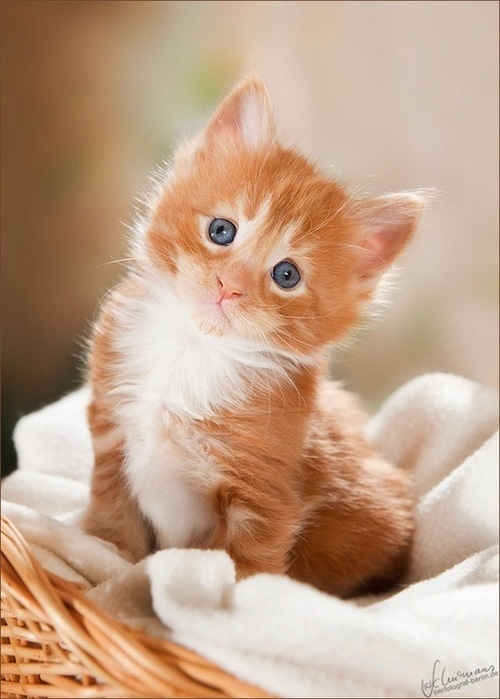
\includegraphics[width=5.5cm, height=5.5cm]{images/CatImage.jpg}};
	\end{scope}
	
	%alexnet
	%\onslide<1->{
	%\cuboidlabel{(0,0,0)}{gray}{0.03}{5.5}{5.5}{3}{227}{227}
	\node (a) at (-0.015-1.5,-6.2,0) {\tiny Input};
	%}
	\onslide<1>{
	\kernellabel{(-1.5,-1,-1)}{blue}{0.03}{1.6}{1.6}{(1.7,-2,-2)}{3}{11}{11}
	}
	\onslide<5->{
	\kernell{(-1.5,-0.7,-1.5)}{green}{0}{3}{3}{(1.7,-2,-2)}
	}
	%\onslide<2>{
	%\node (a) at (-0.015+1,-6.7,0) {\scriptsize $S=4$,$P=0$};
	%\node (a) at (-0.015+1,-7.2,0) {\scriptsize Parameters: $(11\times 11 \times 3)\times 96 = K$};
	%}
	
	
	%\onslide<3->{
	\cuboidlabel{(2,-0.5,-0.5)}{red}{0.6}{4.5}{4.5}{96}{55}{55}
	\node (a) at (2-0.3,-0.5-4.5-0.7,-0.5) {\tiny Convolution};
	%}
	\onslide<1>{
	\kernellabel{(2,-1.5,-1.5)}{blue}{0.6}{0.7}{0.7}{(3.7,-2.5,-2.5)}{96}{3}{3}
	}
	
	\onslide<4->{
	\kernel{(2,-1.5,-1.5)}{green}{0.6}{2}{2}{(3.7,-2.5,-2.5)}
	}
	%\onslide<4>{
	%\node (a) at (2-0.3+1,-6.7,-0.5) {\scriptsize $S=2$,$P=0$};
	%\node (a) at (2-0.3+1,-7.2,-0.5) {\scriptsize Parameters: 0};
	%}
	
	
	%\onslide<5->{
	\cuboidlabel{(4,-1,-1)}{yellow}{0.6}{3.5}{3.5}{96}{27}{27}
	\node (a) at (4-0.3,-1-3.5-0.7,-1) {\tiny MaxPooling};
	%}
	\onslide<1>{
	\kernellabel{(4,-2,-2)}{blue}{0.6}{1}{1}{(5.7,-3,-3)}{96}{5}{5}
	}
	\onslide<3->{
	\kernel{(4,-2,-2)}{green}{0.6}{1}{1}{(5.7,-3,-3)}
	}
	%\onslide<6>{
	%\node (a) at (4-0.3+1,-6.7,-1) {\scriptsize $S=1$,$P=0$};
	%\node (a) at (4-0.3+1,-7.2,-1) {\scriptsize Parameters: $(5\times 5 \times 96)\times 256 = K$};
	%}
	
	
	%\onslide<7->{
	\cuboidlabel{(6,-1.5,-1.5)}{red}{1}{3.3}{3.3}{256}{23}{23}
	\node (a) at (6-0.5,-1.5-3.3-0.7,-1.5) {\tiny Convolution};
	%}
	\onslide<1>{
	\kernellabel{(6,-2.5,-2.5)}{blue}{1}{0.6}{0.6}{(7.7,-3.5,-3.5)}{256}{3}{3}
	}
	
	\onslide<2->{
	\fill[green!50] (6,-2.5,-2.5) ellipse (0.1 and 0.2);
	}
	%\onslide<8>{
	%\node (a) at (6-0.5+1,-6.7,-1.5) {\scriptsize $S=2$,$P=0$};
	%\node (a) at (6-0.5+1,-7.2,-1.5) {\scriptsize Parameters: 0};
	%}
	
	
	%\onslide<9->{
	\cuboidlabel{(8,-2,-2)}{yellow}{1}{2.5}{2.5}{256}{11}{11}
	\node (a) at (8-0.5,-2-2.5-0.7,-2) {\tiny MaxPooling};
	%}
	\onslide<1>{
	\kernellabel{(8,-3,-3)}{blue}{1}{0.6}{0.6}{(9.7,-3.8,-3.8)}{256}{3}{3}
	}
	%\onslide<10>{
	%\node (a) at (8-0.5+1,-6.7,-2) {\scriptsize $S=1$,$P=0$};
	%\node (a) at (8-0.5+1,-7.2,-2) {\scriptsize Parameters: $(3\times 3 \times 256)\times 384 = K$};
	%}
	
	
	%\onslide<11->{
	\cuboidlabel{(10,-2.5,-2.5)}{red}{1.3}{2.2}{2.2}{384}{9}{9}
	\node (a) at (10-0.65,-2.5-2.2-0.7,-2.5) {\tiny Convolution};
	%}
	\onslide<1>{
	\kernellabel{(10,-3.2,-3.2)}{blue}{1.3}{0.6}{0.6}{(11.5,-3.7,-3.7)}{384}{3}{3}
	}
	%\onslide<12>{
	%\node (a) at (10-0.65+1,-6.7,-2.5) {\scriptsize $S=1$,$P=0$};
	%\node (a) at (10-0.65+1,-7.2,-2.5) {\scriptsize Parameters: $(3\times 3 \times 384)\times 384 = K$};
	%}
	
	
	%\onslide<13->{
	\cuboidlabel{(12,-3,-3)}{red}{1.3}{1.5}{1.5}{384}{7}{7}
	\node (a) at (12-0.65,-3-1.5-0.7,-3) {\tiny Convolution};
	%}
	\onslide<1>{
	\kernellabel{(12,-3.5,-3.5)}{blue}{1.3}{0.6}{0.6}{(13,-3.9,-3.9)}{384}{3}{3}
	}
	%\onslide<14>{
	%\node (a) at (12-0.65+1,-6.7,-3) {\scriptsize $S=1$,$P=0$};
	%\node (a) at (12-0.65+1,-7.2,-3) {\scriptsize Parameters: $(3\times 3 \times %384)\times 256 = K$};
	%}
	
	
	%\onslide<15->{
	\cuboidlabel{(13.5,-3.5,-3.5)}{red}{1}{1}{1}{256}{5}{5}
	\node (a) at (13.5-0.5,-3.5-1-0.7,-3.5) {\tiny Convolution};
	%}
	\onslide<1>{
	\kernellabel{(13.5,-3.8,-3.8)}{blue}{1}{0.6}{0.6}{(14,-5.2,-5.2)}{256}{3}{3}
	}
	
	%\onslide<16>{
	%\node (a) at (13.5-0.5+1,-6.7,-3.5) {\scriptsize $S=2$,$P=0$};
	%\node (a) at (13.5-0.5+1,-7.2,-3.5) {\scriptsize Parameters: 0};
	%}
	
	
	
	%\onslide<17->{
	\cuboidlabel{(14.5,-5,-5)}{yellow}{1}{0.5}{0.5}{256}{2}{2}
	\node (a) at (14.5-0.5,-5-0.5-0.7,-5) {\tiny MaxPooling};
	%}
	
	
	%\onslide<18->{
	\draw[dotted,->] (14.5,-5,-5) -- (18,-0.7,0);
	\node (a) at (17.5,0,0) {\tiny dense};
	\cuboid{(18.5,3,0)}{red}{0.5}{7}{0}{256}{2}{2}
	\node (a) at (18.2,-4.5,0) {\tiny 4096};
	%}
	%\onslide<19->{
	\draw[dotted,->] (18.5,-0.7,0) -- (19+0.5,-0.7,0) node[pos=0.5,above] {\tiny dense};
	\cuboid{(19.5+0.5,3,0)}{red}{0.5}{7}{0}{256}{2}{2}
	\node (a) at (19.2+0.5,-4.5,0) {\tiny 4096};
	%}
	
	%\onslide<20->{
	\draw[dotted,->] (19.5+0.5,-0.7,0) -- (20+1,-0.7,0) node[pos=0.5,above] {\tiny dense};
	\cuboid{(20.5+1,2,0)}{red}{0.5}{5}{0}{256}{2}{2}
	\node (a) at (20.2+1,-3.5,0) {\tiny 1000};
	%}
\end{tikzpicture}

